\section{A general overview}
\subsection{Where does it come from?}

\begin{frame}
  \frametitle{The nature}
  \begin{block}{Natural Selection}
    \begin{itemize}
    \item<1-7> Darwin\cite{darwin.1840.origin.of.species} introduces
      Natural selection.
    \item<2-7> It implies several conditions:
      \begin{itemize}
      \item<3-7> Reproduction of individuals in the population.
      \item<4-7> Variation that affects the likelihood of survival of
        individuals.
      \item<5-7> Heredity in reproduction.
      \end{itemize}
    \end{itemize}
  \end{block}

\visible<6-7>{
  \begin{block}{Sexual/Asexual?}
    \begin{itemize}
    \item<6-7> Asexual reproduction is based on cloning, and
      eventually mutation.
    \item<7> Sexual is based on crossover.
    \end{itemize}
  \end{block}
}
\end{frame}

\begin{frame}
  \frametitle{Link with Genetic Programming?}
  \begin{block}{On the idea}
    \begin{itemize}[<+->]
    \item Make evolve a population to solve a problem.
    \item The population could be a lot of things(programs, parameters\dots).
    \end{itemize}
  \end{block}

\invisible<1-2>{
  \begin{block}{On the way its done}
    \begin{itemize}[<+->]
    \item Create the population,
    \item Choose the best,
    \item Keep only the best,
    \item Make them create a new generation,
    \item And so on until the population solves the problem.
    \end{itemize}
  \end{block}
}
\end{frame}


\begin{frame}
  \frametitle{A basis graphical overview}
  \begin{center}
    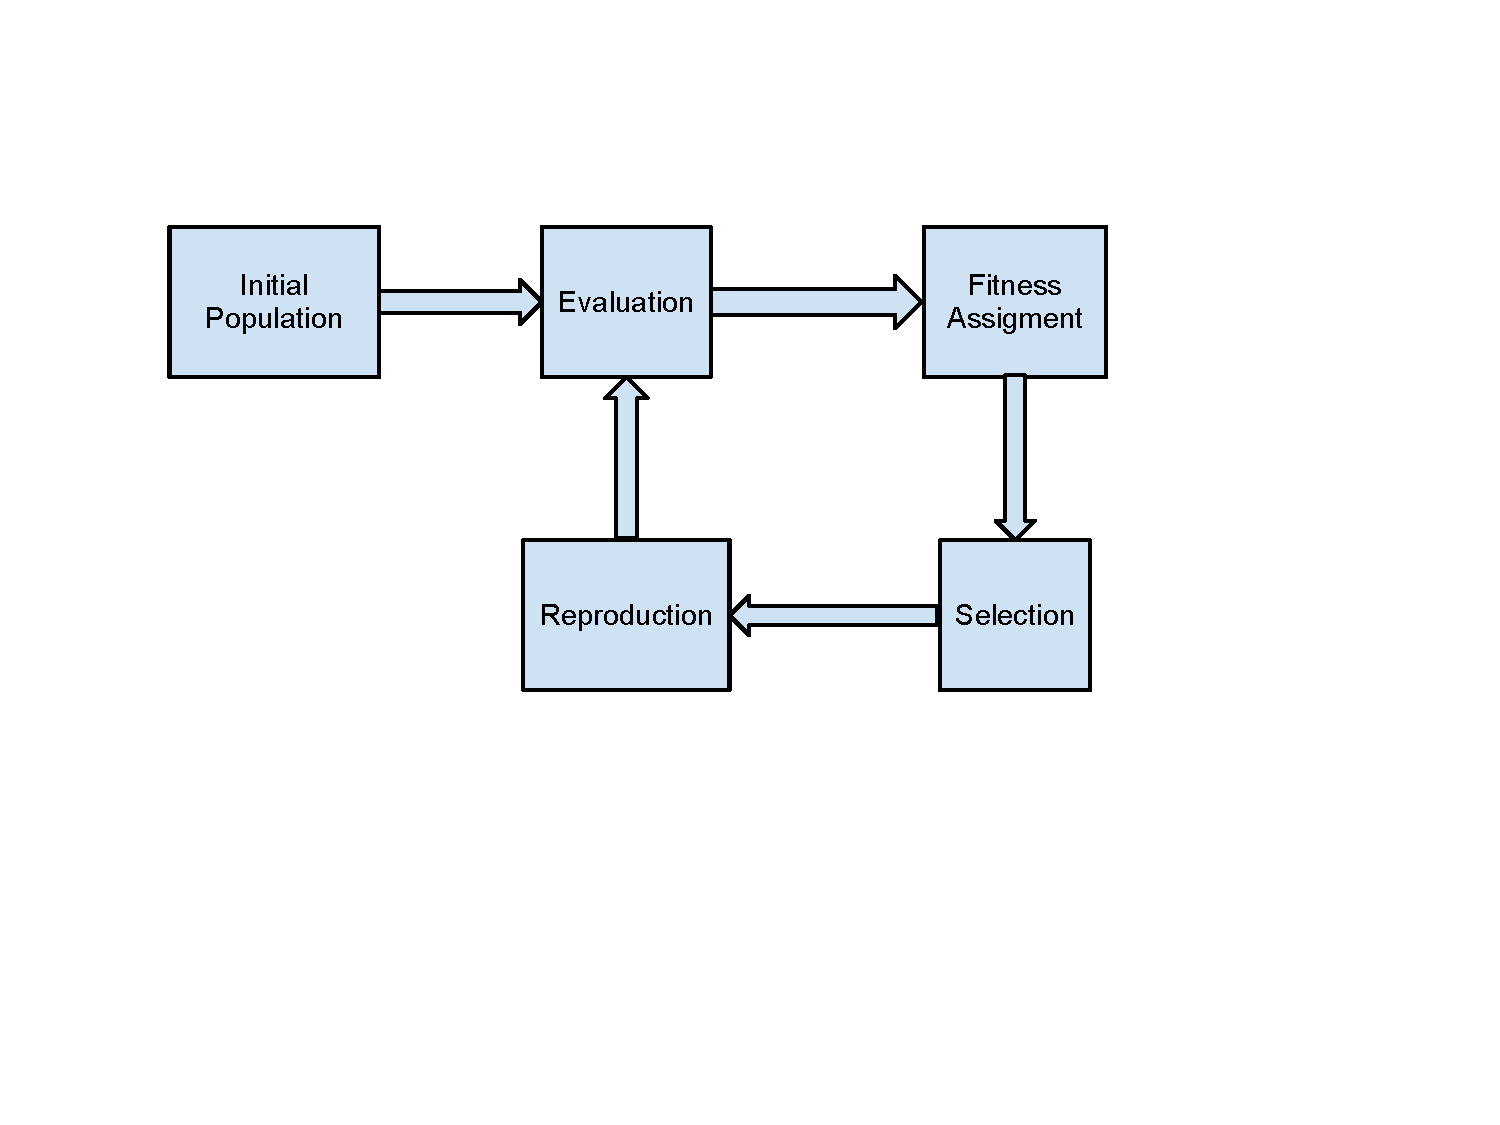
\includegraphics[scale=0.5]{img/cycle}
  \end{center}
\end{frame}

\subsection{Definitions}

\begin{frame}
  \frametitle{EA, GA, GP, ES... ???}
  \begin{block}{In the literature}
    \begin{itemize}[<+->]
    \item When you are looking for genetic programming, you'll find a
      lot of different things.
    \item In this talk, we consider Evolutionary Algorithm as an
      umbrella term to represent techniques which use evolution.
    \end{itemize}
  \end{block}

\visible<3->{
  \begin{center}
    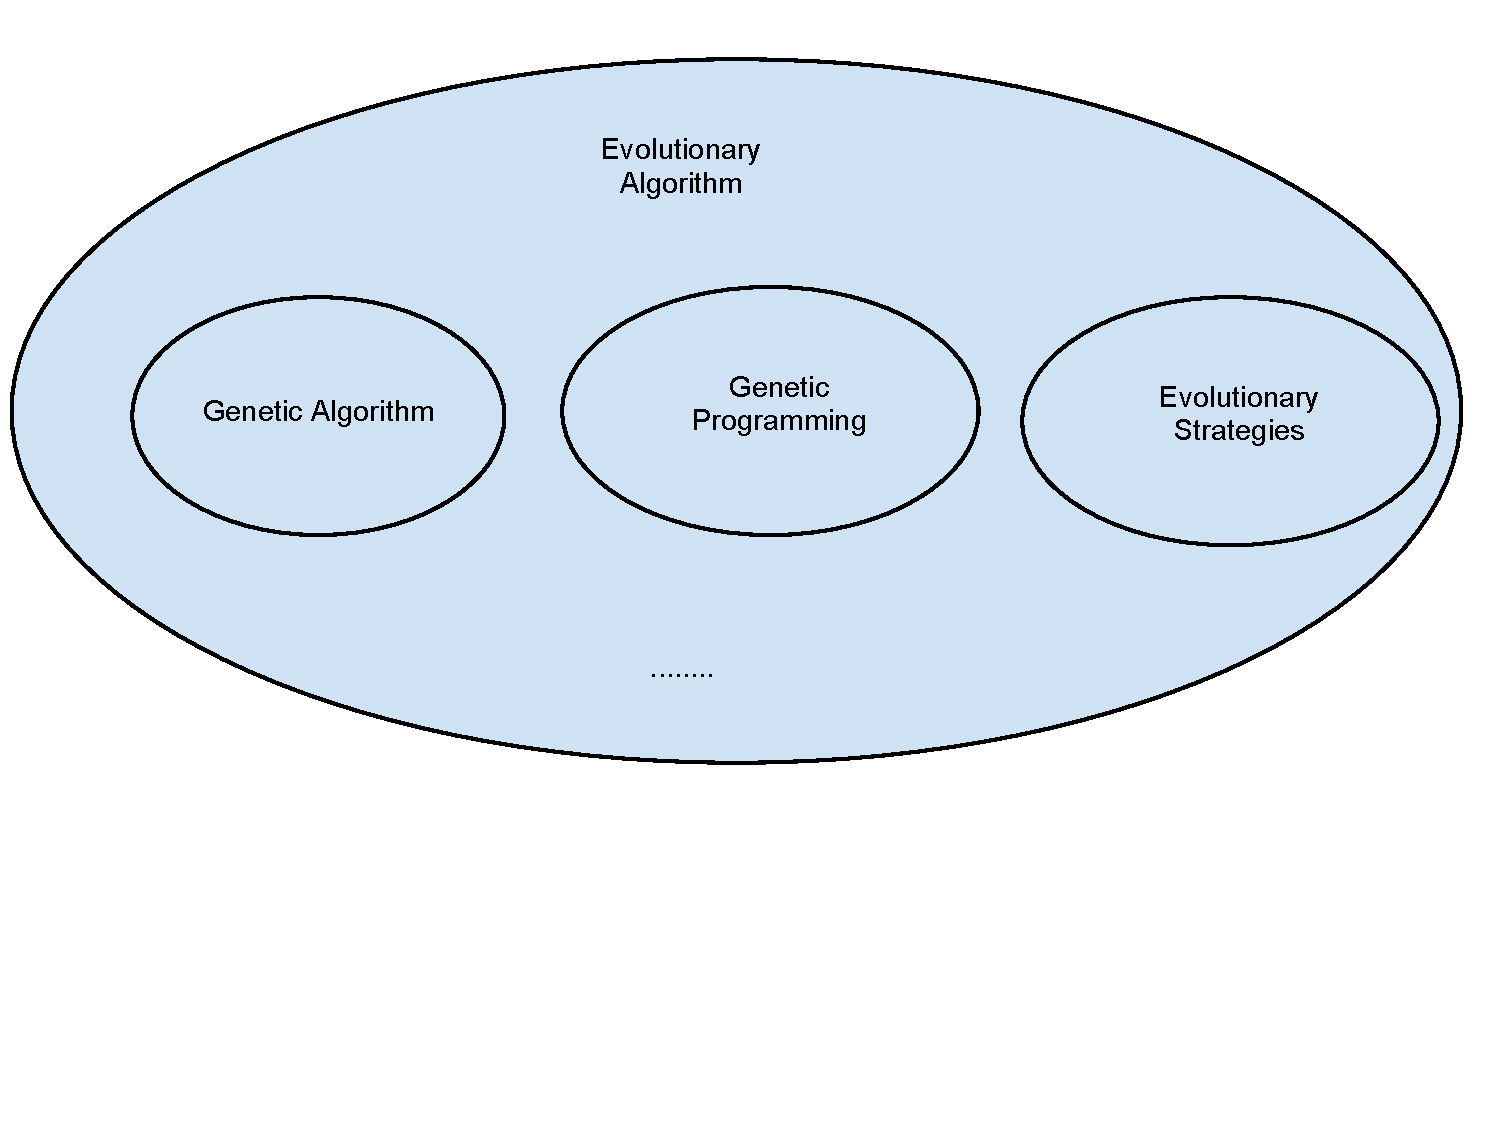
\includegraphics[scale=0.4]{img/ea}
  \end{center}
}
\end{frame}

\begin{frame}
  \frametitle{Genetic Algorithms}
  \begin{block}{History}
    \begin{itemize}[<+->]
    \item Developed by Holland\cite{Holland1992}.
    \item The original GA uses:
      \begin{itemize}[<+->]
        \item fixed-length binary representation.
        \item Crossover a lot.
      \end{itemize}
    \item This model has been extended, now GA uses an alphabet (like DNA).
    \item We'll let the theoretical development for the second part.
      %% In this phrase, I mean Pierre, you have to explain the GA 1-point
      %% crossover (GP An introduction p96) and the schemata.
    \end{itemize}
  \end{block}
\end{frame}

\begin{frame}{Genetic Algorithms (cont.)}
    \begin{algorithmic}
      \State t := 0
      \State initPopulation P(t)
      \State evaluate P(t)
    \end{algorithmic}
\end{frame}

%%% Local Variables:
%%% mode: latex
%%% mode: flyspell
%%% TeX-master: "../genetic"
%%% ispell-dictionary: "en"
%%% compile-command: "cd .. && make"
%%% End:
